\documentclass[border=6pt,tikz]{standalone}
\usepackage{amsmath}
\usepackage{amssymb}
\usepackage{tikz}
\usetikzlibrary{arrows.meta,calc,decorations.pathreplacing,patterns,shapes.geometric,positioning,shadings,decorations.markings,decorations.pathmorphing}

\begin{document}
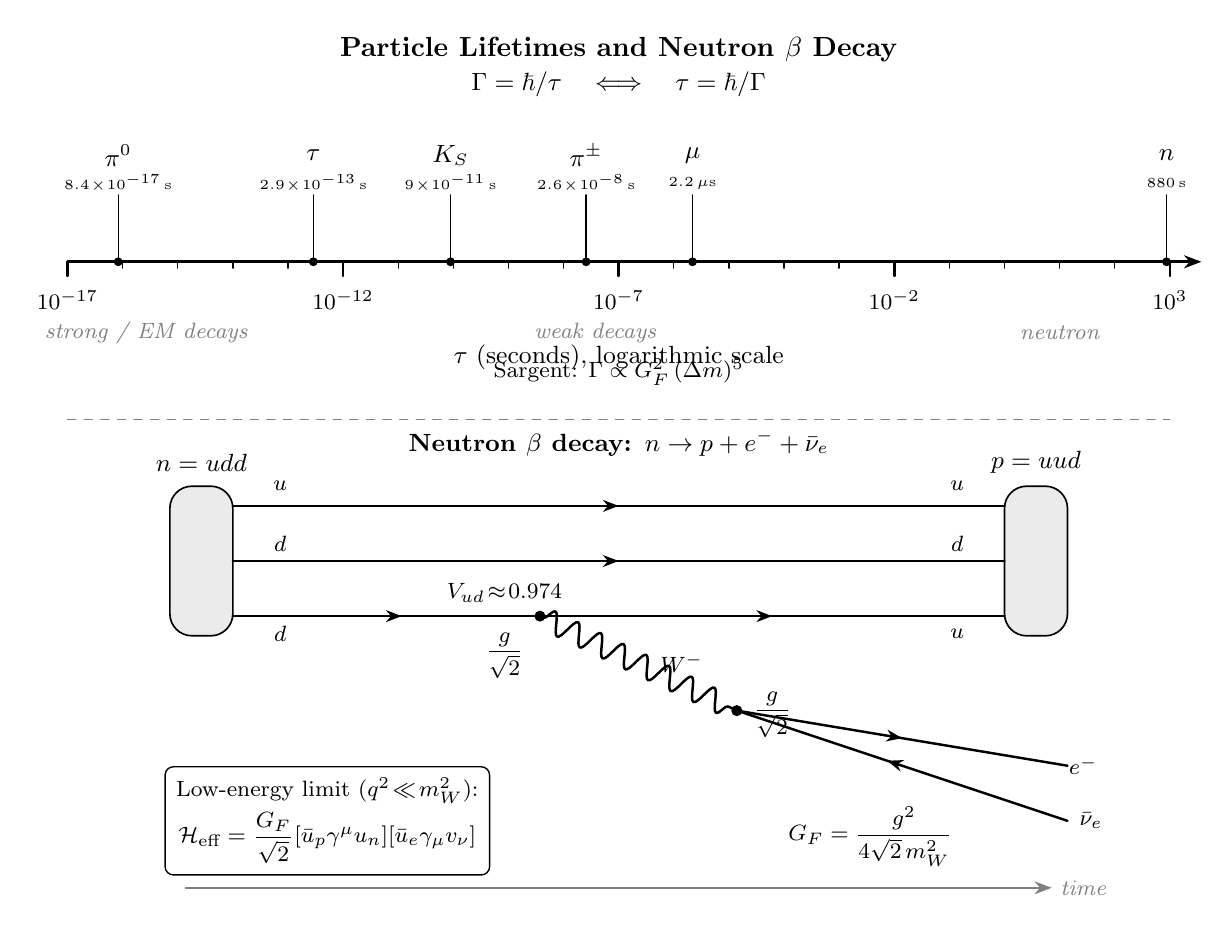
\begin{tikzpicture}[
    >={Stealth[length=2.2mm]},
    line cap=round,
    line join=round,
    every node/.style={font=\small}
]

% =====================================================================
% Title
% =====================================================================
\node[font=\bfseries] at (7,8.4) {Particle Lifetimes and Neutron $\beta$ Decay};
\node[font=\small\itshape] at (7,7.95) {$\Gamma=\hbar/\tau \quad\Longleftrightarrow\quad \tau=\hbar/\Gamma$};

% =====================================================================
% TOP: log time axis from 10^-17 to 10^3
% Map x in [0, 14] -> log10(t) in [-17, 3]; step 0.7 per decade
% =====================================================================
\def\xMin{0}
\def\xMax{14}
\def\yAxis{5.7}

% Helper: position for an exponent k in [-17,3]
% xpos = (k - (-17)) * 0.7

% Main axis line
\draw[line width=1pt,black] (\xMin,\yAxis) -- (\xMax,\yAxis);
\draw[->,line width=1pt,black] (\xMax,\yAxis) -- (\xMax+0.4,\yAxis);

% Major ticks every 5 decades: -17, -12, -7, -2, 3
\foreach \k in {-17,-12,-7,-2,3}{
  \pgfmathsetmacro{\xpos}{(\k+17)*0.7}
  \draw[line width=0.9pt] (\xpos,\yAxis) -- (\xpos,\yAxis-0.18);
  \node[below=2pt,font=\footnotesize] at (\xpos,\yAxis-0.18) {$10^{\k}$};
}

% Minor ticks every decade
\foreach \k in {-17,-16,-15,-14,-13,-12,-11,-10,-9,-8,-7,-6,-5,-4,-3,-2,-1,0,1,2,3}{
  \pgfmathsetmacro{\xpos}{(\k+17)*0.7}
  \draw[line width=0.5pt] (\xpos,\yAxis) -- (\xpos,\yAxis-0.08);
}

% Axis label
\node[below=18pt,font=\small] at (\xMax/2,\yAxis-0.3) {$\tau$ (seconds), logarithmic scale};

% Particle markers (placed above axis with leader lines)
% pi^0 at 8.4e-17 -> log = -16.08
% tau at 2.9e-13 -> log = -12.54
% K_S at 0.9e-10 -> log = -10.05
% pi+- at 2.6e-8 -> log = -7.59
% mu  at 2.2e-6 -> log = -5.66
% n   at 880    -> log =  2.94

\def\markY{6.55}
\def\labY{7.05}

% pi0
\pgfmathsetmacro{\xPi}{(-16.08+17)*0.7}
\fill[black] (\xPi,\yAxis) circle (1.6pt);
\draw[line width=0.5pt] (\xPi,\yAxis) -- (\xPi,\markY);
\node[font=\small,fill=white,inner sep=1pt] at (\xPi,\labY) {$\pi^{0}$};
\node[font=\tiny,fill=white,inner sep=0.5pt] at (\xPi,\labY-0.35) {$8.4\!\times\!10^{-17}\,\mathrm{s}$};

% tau
\pgfmathsetmacro{\xTau}{(-12.54+17)*0.7}
\fill[black] (\xTau,\yAxis) circle (1.6pt);
\draw[line width=0.5pt] (\xTau,\yAxis) -- (\xTau,\markY);
\node[font=\small,fill=white,inner sep=1pt] at (\xTau,\labY) {$\tau$};
\node[font=\tiny,fill=white,inner sep=0.5pt] at (\xTau,\labY-0.35) {$2.9\!\times\!10^{-13}\,\mathrm{s}$};

% K_S
\pgfmathsetmacro{\xKS}{(-10.05+17)*0.7}
\fill[black] (\xKS,\yAxis) circle (1.6pt);
\draw[line width=0.5pt] (\xKS,\yAxis) -- (\xKS,\markY);
\node[font=\small,fill=white,inner sep=1pt] at (\xKS,\labY) {$K_{S}$};
\node[font=\tiny,fill=white,inner sep=0.5pt] at (\xKS,\labY-0.35) {$9\!\times\!10^{-11}\,\mathrm{s}$};

% pi+-
\pgfmathsetmacro{\xPiC}{(-7.59+17)*0.7}
\fill[black] (\xPiC,\yAxis) circle (1.6pt);
\draw[line width=0.5pt] (\xPiC,\yAxis) -- (\xPiC,\markY);
\node[font=\small,fill=white,inner sep=1pt] at (\xPiC,\labY) {$\pi^{\pm}$};
\node[font=\tiny,fill=white,inner sep=0.5pt] at (\xPiC,\labY-0.35) {$2.6\!\times\!10^{-8}\,\mathrm{s}$};

% mu
\pgfmathsetmacro{\xMu}{(-5.66+17)*0.7}
\fill[black] (\xMu,\yAxis) circle (1.6pt);
\draw[line width=0.5pt] (\xMu,\yAxis) -- (\xMu,\markY);
\node[font=\small,fill=white,inner sep=1pt] at (\xMu,\labY) {$\mu$};
\node[font=\tiny,fill=white,inner sep=0.5pt] at (\xMu,\labY-0.35) {$2.2\,\mu\mathrm{s}$};

% n
\pgfmathsetmacro{\xN}{(2.94+17)*0.7}
\fill[black] (\xN,\yAxis) circle (1.6pt);
\draw[line width=0.5pt] (\xN,\yAxis) -- (\xN,\markY);
\node[font=\small,fill=white,inner sep=1pt] at (\xN,\labY) {$n$};
\node[font=\tiny,fill=white,inner sep=0.5pt] at (\xN,\labY-0.35) {$880\,\mathrm{s}$};

% Region labels
\node[font=\footnotesize\itshape,gray] at (1.0,4.8) {strong / EM decays};
\node[font=\footnotesize\itshape,gray] at (6.7,4.8) {weak decays};
\node[font=\footnotesize\itshape,gray] at (12.6,4.8) {neutron};

% Sargent rule annotation
\node[font=\footnotesize] at (\xMax/2,4.3) {Sargent: $\Gamma\propto G_F^{2}\,(\Delta m)^{5}$};

% =====================================================================
% Separator
% =====================================================================
\draw[dashed,gray] (\xMin,3.7) -- (\xMax,3.7);
\node[font=\small\bfseries] at (7,3.4) {Neutron $\beta$ decay: $n \to p + e^{-} + \bar\nu_{e}$};

% =====================================================================
% BOTTOM: Feynman diagram
% Time flows left to right
% Three quark lines for n (udd) on left, become p (uud) on right
% A d quark emits W^- which decays to e^- + nubar
% =====================================================================

% Coordinates
\def\xL{1.5}     % left edge
\def\xR{12.5}    % right edge
\def\xV{6.0}     % vertex x of d -> u + W^-
\def\yUq{2.6}    % u quark line y
\def\yDa{1.9}    % first d quark line y
\def\yDb{1.2}    % second d quark line y
\def\xW{8.5}     % W decay vertex x
\def\yW{0.0}     % W endpoint y
\def\yE{-0.7}    % electron y
\def\yNu{-1.4}   % antineutrino y

% Hadron blobs (n on left, p on right)
\draw[fill=black!8,line width=0.6pt,rounded corners=8pt]
  (\xL-0.2,\yDb-0.25) rectangle (\xL+0.6,\yUq+0.25);
\node[font=\small\bfseries] at (\xL+0.2,\yUq+0.55) {$n=udd$};

\draw[fill=black!8,line width=0.6pt,rounded corners=8pt]
  (\xR-0.6,\yDb-0.25) rectangle (\xR+0.2,\yUq+0.25);
\node[font=\small\bfseries] at (\xR-0.2,\yUq+0.55) {$p=uud$};

% Spectator quark u (top) - straight line through
\draw[line width=0.9pt,
      decoration={markings, mark=at position 0.5 with {\arrow{Stealth[length=2mm]}}},
      postaction={decorate}]
  (\xL+0.6,\yUq) -- (\xR-0.6,\yUq);
\node[font=\footnotesize] at (\xL+1.2,\yUq+0.25) {$u$};
\node[font=\footnotesize] at (\xR-1.2,\yUq+0.25) {$u$};

% Spectator quark d (middle) - straight line through
\draw[line width=0.9pt,
      decoration={markings, mark=at position 0.5 with {\arrow{Stealth[length=2mm]}}},
      postaction={decorate}]
  (\xL+0.6,\yDa) -- (\xR-0.6,\yDa);
\node[font=\footnotesize] at (\xL+1.2,\yDa+0.22) {$d$};
\node[font=\footnotesize] at (\xR-1.2,\yDa+0.22) {$d$};

% d -> u with vertex emitting W^-
\draw[line width=0.9pt,
      decoration={markings, mark=at position 0.55 with {\arrow{Stealth[length=2mm]}}},
      postaction={decorate}]
  (\xL+0.6,\yDb) -- (\xV,\yDb);
\node[font=\footnotesize] at (\xL+1.2,\yDb-0.22) {$d$};

\draw[line width=0.9pt,
      decoration={markings, mark=at position 0.5 with {\arrow{Stealth[length=2mm]}}},
      postaction={decorate}]
  (\xV,\yDb) -- (\xR-0.6,\yDb);
\node[font=\footnotesize] at (\xR-1.2,\yDb-0.22) {$u$};

% Vertex dots
\fill[black] (\xV,\yDb) circle (2pt);
\fill[black] (\xW,\yW) circle (2pt);

% W^- boson line (wavy) from quark vertex down-right to lepton vertex
\draw[line width=0.9pt, decorate, decoration={snake, amplitude=1.4mm, segment length=3.2mm, post length=0.5mm, pre length=0.5mm}]
  (\xV,\yDb) -- (\xW,\yW);
\node[font=\footnotesize] at ($(\xV,\yDb)!0.5!(\xW,\yW)+(0.55,0.0)$) {$W^{-}$};

% V_ud label near quark vertex
\node[font=\footnotesize] at (\xV-0.45,\yDb+0.30) {$V_{ud}\!\approx\!0.974$};
\node[font=\footnotesize] at (\xV-0.45,\yDb-0.50) {$\dfrac{g}{\sqrt{2}}$};

% Electron line from W vertex to lower right
\draw[line width=0.9pt,
      decoration={markings, mark=at position 0.5 with {\arrow{Stealth[length=2mm]}}},
      postaction={decorate}]
  (\xW,\yW) -- (\xR+0.2,\yE);
\node[font=\footnotesize] at (\xR+0.4,\yE) {$e^{-}$};

% Antineutrino line from W vertex (anti-particle: arrow reversed - arrow points back to vertex)
\draw[line width=0.9pt,
      decoration={markings, mark=at position 0.5 with {\arrow{Stealth[length=2mm,reversed]}}},
      postaction={decorate}]
  (\xW,\yW) -- (\xR+0.2,\yNu);
\node[font=\footnotesize] at (\xR+0.5,\yNu) {$\bar\nu_{e}$};

% Vertex coupling at W decay
\node[font=\footnotesize] at (\xW+0.45,\yW-0.05) {$\dfrac{g}{\sqrt{2}}$};

% Time arrow at bottom
\draw[->,line width=0.6pt,gray] (\xL,-2.25) -- (\xR,-2.25);
\node[font=\footnotesize\itshape,gray] at (\xR+0.4,-2.25) {time};

% Effective vertex annotation (Fermi 4-fermion limit)
\node[draw,rounded corners=3pt,line width=0.5pt,inner sep=4pt,
      align=center,font=\footnotesize] at (3.3,-1.4)
  {Low-energy limit ($q^{2}\!\ll\! m_{W}^{2}$):\\[2pt]
   $\mathcal{H}_{\text{eff}}=\dfrac{G_{F}}{\sqrt{2}}[\bar u_{p}\gamma^{\mu}u_{n}][\bar u_{e}\gamma_{\mu}v_{\nu}]$};

\node[font=\footnotesize] at (10.2,-1.6) {$G_{F}=\dfrac{g^{2}}{4\sqrt{2}\,m_{W}^{2}}$};

\end{tikzpicture}
\end{document}
